\documentclass[12pt]{article}
% Full article preamble (duplicated, no common file)
\usepackage{fontspec}
\usepackage[a4paper,margin=2.5cm,includefoot]{geometry}
\usepackage{polyglossia}
\usepackage{amsmath}
\usepackage{amssymb}
\usepackage{xcolor}
\usepackage{fancyhdr}
\usepackage{graphicx}
\usepackage{listings}
\usepackage[most]{tcolorbox}
\usepackage{pifont}
\usepackage{enumitem}
\usepackage{titlesec}
\usepackage[bottom]{footmisc}
\usepackage{titling}
\usepackage{minted}
\usepackage{etoolbox}
\usepackage{array}
\usepackage{extsizes}

\newfontfamily\emoji{Segoe UI Emoji}

\pagestyle{fancy}

\setmainlanguage[numerals=western]{arabic}
\setotherlanguage{english}
\newfontfamily\arabicfont[Script=Arabic]{Amiri}
\newfontfamily\arabicfonttt[Script=Arabic]{Courier New}

\lstset{
  language=[Sharp]C,
  numbers=left,
  stepnumber=1,
  numbersep=8pt,
  frame=single,
  basicstyle=\ttfamily\small,
  keywordstyle=\color{blue},
  stringstyle=\color{red},
  commentstyle=\color{green!50!black}
}

\newif\ifdetailed
\ifdefined\setdetailed
  \setdetailed
\fi

\newif\ifwithsols
\ifdefined\setwithsols
  \setwithsols
\fi

% unified tcolorboxes for articles
\tcbset{colback=white, colframe=black, fonttitle=\bfseries, boxrule=0.8pt}
\newtcolorbox{boxDef}[1][]{colback=blue!5!white,colframe=blue!75!black,
  title={{\emoji📘} تعريف\ifx\\#1\\\else ~#1\fi :}}
\newtcolorbox{boxExercise}[1][]{colback=cyan!5!white,colframe=cyan!70!black,
  title={{\emoji🧩} تمرين\ifx\\#1\\\else ~#1\fi :}}
\newtcolorbox{boxExample}[1][]{colback=yellow!5!white,colframe=orange!90!black,
  title={{\emoji📝} مثال\ifx\\#1\\\else ~#1\fi :}}
\newtcolorbox{boxNote}[1][]{colback=gray!10!white,colframe=black,
  title={{\emoji✨} ملاحظة\ifx\\#1\\\else ~#1\fi :}}
\newtcolorbox{boxAttention}[1][]{colback=magenta!10!white,colframe=magenta!80!black,
  title={{\emoji🔔} تنبيه\ifx\\#1\\\else ~#1\fi :}}
\newtcolorbox{boxWarning}[1][]{colback=red!5!white,colframe=red!75!black,
  title={{\emoji⚡} ملاحظة هامة\ifx\\#1\\\else ~#1\fi :}}
\newtcolorbox{boxSolution}[1][]{colback=green!5!white,colframe=green!60!black,
  title={{\emoji✅} حل\ifx\\#1\\\else ~#1\fi :}}
\newtcolorbox{boxSymbol}[1][]{colback=purple!5!white,colframe=purple!70!black,
  title={{\emoji🔣} رمز\ifx\\#1\\\else ~#1\fi :}}

\tcbset{simplecode/.style={ colback=gray!5, colframe=black!50, boxrule=0.4pt, arc=2pt, left=4pt,right=4pt,top=4pt,bottom=4pt}}
\newenvironment{boxCode}{\begin{tcolorbox}[simplecode]}{\end{tcolorbox}}

\newcolumntype{C}[1]{>{\centering\arraybackslash}p{#1}}

% redefine spaces after titles
\makeatletter
\renewcommand{\@maketitle}{%
  \begin{center}
    {\huge \bfseries \@title \par}%
    \vskip 0.2em % space between title and author
    {\large \@author \par}%
    % \vskip 0.2em % space between author and date
    % {\normalsize \@date \par}%
  \end{center}
}
\makeatother

\fancyhf{} % clear default
\fancypagestyle{plain}{
  \fancyhf{}
  \fancyhead[L]{مدرسة التسامح الشاملة}
  % \fancyhead[L]{
\includegraphics[height=1cm]{../../../images/logoTasamoh.png}}
  \fancyhead[R]{الأستاذ محمود اغبارية}
  \fancyfoot[C]{\thepage}
}

\fancyhead[L]{مدرسة التسامح الشاملة}
\fancyhead[R]{الأستاذ محمود اغبارية}
\fancyfoot[C]{\thepage}
% \date{\today}

\setcounter{tocdepth}{3} % only section subsection and subsubsection in TOC


% ----------------------


% \begin{document}

% \maketitle

% % \clearpage  % start TOC on a new page
% % \renewcommand{\contentsname}{جدول المحتويات}
% % \tableofcontents
% % \clearpage

% \part*{part 1} % the * prevents numbering
% \section*{مقدمة}
% \subsection*{مثال رياضي}
% \subsubsection*{مثال فرعي}
% \paragraph*{ paragraph 1}
% \subparagraph*{sub paragraph 1}

% \ifdetailed
% \begin{english}
% \begin{minted}{csharp}
% // C# Example
% \end{minted}
% \end{english}
% \fi

% OLD WAY
% \ifdetailed
% \begin{english}
% \begin{lstlisting}
% // C# Example
% \end{lstlisting}
% \end{english}
% \fi

% % 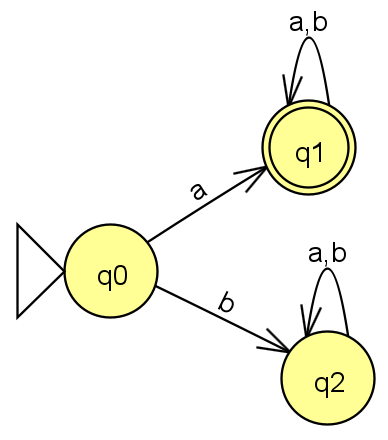
\includegraphics[width=0.2\textwidth]{../../../images/DFAs/ex1_q1.png}



% \vspace{3cm}
% \begin{flushleft}
% أرجو لكم وقتًا ممتعًا.

% الأستاذ محمود اغبارية.
% \end{flushleft}


% \end{document}


\title{وظيفة 1 للصف 11-10 - مجموعات ولغات}

\begin{document}

\maketitle

\textbf{1. السؤال الأول:} نعرّف اللغات التالية:
\begin{align*}
    L_1 &= \{a^n b^n \mid n \geq 1\} \\
    L_2 &= \{a^n b^m \mid n,m \geq 1\} \\
    L_3 &= \{a^n b^m \mid n,m \geq 0\}
\end{align*}

لكل واحد من الادّعاءات التالية اكتب هل هو صحيح أم لا.
\begin{enumerate}
\item $L_1 \subseteq L_2$
\item $L_2 \subseteq L_3$
\item $L_3 \subseteq L_1$
\item $\epsilon \in L_1$
\item $\epsilon \in L_2$
\item $\epsilon \in L_3$
\item $aa \in L_1$
\item $aa \in L_2$
\item $aa \in L_3$
\item $b \in L_3$
\item $ba \in L_2$
\item $abb \in L_1$
\item $abb \in L_2$
\item $abb \in L_3$
\end{enumerate}

\ifwithsols
\clearpage
\begin{boxSolution}
\begin{enumerate}
\item صحيح
\item صحيح
\item خطأ
\item خطأ
\item خطأ
\item صحيح
\item خطأ
\item خطأ
\item صحيح
\item صحيح
\item خطأ
\item خطأ
\item صحيح
\item صحيح
\end{enumerate}
\end{boxSolution}
\fi

\clearpage
\textbf{2. السؤال الثاني:} أي اللغات التالية مساوية للغة $L = {a^* \cdot a \cdot a^*}$ ؟ \\
اختر جميع الإجابات الصحيحة (هناك أكثر من إجابة صحيحة)

\begin{enumerate}
    \item $L_1 = {a^*}$
    \item $L_2 = {a^* \cdot a}$
    \item $L_3 = {a \cdot a^*}$
    \item $L_4 = {a^+}$
    \item $L_5 = {a \cdot a^+}$
    \item $L_6 = \{a^n \mid n \geq 0\}$
    \item $L_7 = \{a^n \mid n > 0\}$
\end{enumerate}


\ifwithsols
\begin{boxSolution}
    اللغة $L$ هي لغة كل الكلمات المكونة من الحرف $a$ فقط، بحيث يظهر الحرف $a$ مرة واحدة على الأقل.
    \begin{enumerate}
        \item غير مساوية، لأنّ $\epsilon \in L1$ ولكن $\epsilon \notin L$
        \item مساوية
        \item مساوية
        \item مساوية
        \item غير مساوية، لأنّ $a \notin L5$ بينما $a \in L$
        \item غير مساوية، لأنّ $\epsilon \in L6$ ولكن $\epsilon \notin L$
        \item مساوية
    \end{enumerate}
\end{boxSolution}
\clearpage
\fi

\textbf{3. السؤال الثالث:} أمامكم ست لغات فوق الأبجدية $\Sigma = \{0,1\}$:
\begin{align*}
    L_1 &= \emptyset \\
    L_2 &= \Sigma^* \\
    L_3 &= \{\epsilon\} \\
    L_4 &= \{0110\} \\
    L_5 &= \{\epsilon, 110, 00\} \\
    L_6 &= \{1, 0110, 110, 01\}
\end{align*}

اكتبوا اللغة التي تنتج من كل واحدة من العمليات التالية:

\begin{enumerate}
    \item $L_1 \cap L_2$
    \item $L_1 \cup L_2$
    \item $L_1 \cup L_3$
    \item $L_2 \cup L_3$
    \item $L_5 \cap L_6$
    \item $L_5 \cup L_6$
    \item $L_3 \cdot L_4$
    \item $L_4 \cdot L_5$
    \item $L_1 \cdot L_6$
\end{enumerate}

\ifwithsols
\begin{boxSolution}
    \begin{enumerate}
        \item
        $L_1 \cap L_2 = \emptyset$

        \item
        $L_1 \cup L_2 = \Sigma^*$

        \item
        $L_1 \cup L_3 = \{\epsilon\}$

        \item
        $L_2 \cup L_3 = \Sigma^*$

        \item
        $L_5 \cap L_6 = \{110\}$

        \item
        $L_5 \cup L_6 = \{\epsilon, 110, 00, 1, 0110, 01\}$

        \item
        $L_3 \cdot L_4 = \{0110\}$

        \item
        $L_4 \cdot L_5 = \{0110, 0110110, 011000\}$

        \item
        $L_1 \cdot L_6 = \emptyset$
    \end{enumerate}
\end{boxSolution}
\fi

\vspace{1.5cm}
\begin{flushleft}
أرجو لكم وقتًا ممتعًا.

الأستاذ محمود اغبارية.
\end{flushleft}

\end{document}
